\documentclass{article}
\usepackage{booktabs}
\usepackage[T1]{fontenc}
\usepackage{mathtools}
\usepackage[UKenglish]{babel}
\usepackage[UKenglish]{isodate}
\usepackage{fullpage}
\usepackage{graphicx}
\usepackage{hyperref}
\usepackage{listings}
\usepackage{subcaption}
\usepackage{tikz-uml}
\usepackage[binary-units = true]{siunitx}
\usepackage[ruled, vlined]{algorithm2e}

\title{Automated Benchmarking of Container Applications}
\author{Paulius Dilkas}

\begin{document}
\maketitle

%\begin{abstract}
%\end{abstract}

\section{Introduction}

Before an application is deployed to a cloud, one needs to select the required
number of resources. But what is the right resource configuration for \emph{my}
application? One might ask and wonder whether there is a way to obtain a clear
answer.

We present a benchmarking system that can simulate the workflow of a range of
distributed applications, measure various performance metrics, and detect
whether a given resource configuration is sufficient for the application to
perform well.

The system comes with a number of predefined configuration files that represent
realistic workloads of common applications. Every aspect of each configuration
file can be adjusted, and new configuration files can be created to represent,
e.g., additional components of the application.

Our simulated applications consist of a sequence of maps implemented using
Apache Flink. They receive messages from a \emph{control server} and perform a
predefined amount of work, using a predefined amount of memory. The server can
send any number messages at specified intervals (or in more interesting
patterns, if I get around to implementing that).

The Flink application is enclosed in a Docker container and deployed on the
OpenShift cloud platform. Performance metrics are recorded using Prometheus,
which is assumed to be a separate application deployed on the same OpenShift
platform.

\section{Architecture and Implementation}

In this section we describe implementation details of the system at its current
state. During the first stage of the project, the system was deployed and tested
on MiniShift---a single-node OpenShift implementation. While the intent is to
progress to an OpenShift cloud, some of the current implementation details are
specific to MiniShift.

In Section~\ref{sec:deployment} we describe our initial Docker
container-based configuration and how it was transformed into \emph{manifestos},
i.e., OpenShift deployment configuration files. We also discuss modifications to
the standard Prometheus deployment on MiniShift as well as configuration files
that can be used to simulate various applications, add new performance metrics,
etc. In Section~\ref{sec:execution} we dive into Java code to explain what
happens during execution: how the Flink app interacts with the control server
and simulates work and how performance metrics are tracked and recorded.

\subsection{Deployment} \label{sec:deployment}

Flink deployment consists of a JobManager that manages the work, one or more
TaskManagers that execute tasks, and a command that tells JobManager what to do.
In order to deploy these services on OpenShift, we need to put each `work unit'
(something that can run on a separate node) in its own Docker container. We
ended up using two simple Dockerfiles.

The first one is used for both TaskManagers and the JobManager and extends the
original Flink Docker image by enabling Prometheus support on port 9250.
Prometheus can then use that port to retrieve and record performance metrics.

The second Dockerfile extends the first one by adding a JAR file with Java code
for both the control server and the Flink app. This image also contains a custom
\texttt{ENTRYPOINT} shell script that sends the Flink app to the JobManager (via
port 8081) as a background process, while executing the control server in the
foreground. This is the optimal arrangement of the two processes since the
control server always waits for the Flink app to finish in order to take its
running time into account when requesting data from Prometheus.

In both Dockerfiles, one needs to change the permissions and group ownership of the
\texttt{/opt/flink} directory (to \texttt{775} and \texttt{root} respectively)
so that the containers can be successfully executed by any user belonging to the
group \texttt{root}. Both images were put on Docker Hub in order to make them
easily accessible by MiniShift.

A Docker Compose file can then be used to combine several Dockerfiles into a
valid deployment configuration. In this file we define three services:
\texttt{Control}, \texttt{JobManager}, and \texttt{TaskManager}, establishing
open ports as pictured in Figure~\ref{fig:uml}. This file was then converted to
OpenShift manifestos using Kompose\footnote{\url{http://kompose.io/}}. The
generated manifestos, relevant network connections, and other dependencies are
displayed in Figure~\ref{fig:uml}. A notable difference between the two
configurations is that while a Docker Compose file defines only services,
OpenShift has both services and pods. \emph{Service} manifestos define the
network interface (i.e., what ports are open), while manifestos for \emph{pods}
contain the details of what Docker containers should be run, restart policy,
additional data that should be mounted to the pod, etc. The entire system can
then be updated and deployed by generating a new JAR file using Maven, building
and uploading the two Dockerfiles, and recreating all components of the
OpenShift configuration, as described by the manifestos.

% deployment of configuration files
Configuration Files component in Figure~\ref{fig:uml} represents a
\texttt{ConfigMap} OpenShift entity created using the \texttt{oc} command that
contains two configuration files, \texttt{global.yaml} and
\texttt{components.yaml} (see Figures \ref{fig:global} and \ref{fig:components}
for examples). The former contains basic networking information along with three
parameters that control the experiment as well as a list of metrics.
The experiment-specific parameters control how often to send messages
(\texttt{messagesPerSecond}), how long the experiment should last
(\texttt{experimentLength}), and how many messages to send at a time
(\texttt{requestsPerMessage}). Each metric is described with three properties:
\texttt{name}, \texttt{filename}, and \texttt{query}. The last one corresponds
to the name of the property as defined by Prometheus, while the other two are
used for data storage and plotting. The \texttt{components.yaml} configuration
file, on the other hand, describes a sequence of processing stages (maps), each
with its own CPU usage time, memory usage, and output data size (i.e., the
amount of data passed to the next stage).

% local Prometheus setup
Lastly, it is worth mentioning that the Prometheus add-on for
MiniShift\footnote{\url{https://github.com/minishift/minishift-addons/tree/master/add-ons/prometheus}}
had to be modified in order to disable OAuth-based authentication by replacing
\[
  \texttt{-skip-auth-regex=\^{}/metrics} \quad \text{with} \quad
  \texttt{-skip-auth-regex=\^{}/}.
\]
This may or may not be a problem when moving from MiniShift to an actual cloud.
Furthermore, Prometheus configuration file was updated to set both scrape and
evaluation intervals to \SI{1}{\second} and the list of targets to JobManager
and TaskManager, both on port 9250.

\begin{figure}
  \centering
  \begin{tikzpicture}
    % components: first column
    \umlbasiccomponent[x=-6, y=3, fill=cyan!20]{Prometheus}
    \begin{umlcomponent}[fill=cyan!20]{Configuration Files}
      \umlbasiccomponent[x=-6, y=-2, fill=red!20]{Global}
      \umlbasiccomponent[x=-6, y=-4, fill=red!20]{Components}
    \end{umlcomponent}

    % components: second column
    \umlbasiccomponent[x=0, y=1]{Control Service}
    \begin{umlcomponent}{Control Pod}
      \umlbasiccomponent[x=0, y=-2, fill=red!20]{Control Server}
      \umlbasiccomponent[x=0, y=-4, fill=red!20]{Benchmarker}
    \end{umlcomponent}
    \umlbasiccomponent[x=0, y=-7]{Control Persistent Volume Claim}
    \umlbasiccomponent[x=0, y=-10]{Control Persistent Volume}

    % components: third column
    \umlbasiccomponent[x=6, y=3]{JobManager Service}
    \umlbasiccomponent[x=6, y=-1]{JobManager Pod}
    \umlbasiccomponent[x=6, y=-4]{TaskManager Service}
    \umlbasiccomponent[x=6, y=-8]{TaskManager Pod}

    % connections in second column
    \umlVHVassemblyconnector{Control Persistent Volume Claim}{Control Persistent Volume}
    \umlVHVassemblyconnector{Control Pod}{Control Persistent Volume Claim}
    \umlprovidedinterface[interface=998, with port, distance=2.5]{Control Server}
    \umlrequiredinterface[interface=998, with port]{Benchmarker}
    \umlHVassemblyconnector{Control Service}{Control Server-west-interface}
    \umlHVassemblyconnector{Control Service}{Benchmarker-east-interface}

    % connections between first and second columns
    \umlHVHassemblyconnector[interface={\space}, arm1=-2.3]{Benchmarker}{Global}
    \umlVHVassemblyconnector[interface={\space}]{Control Server}{Global}
    \umlVHVassemblyconnector[interface={\space}, arm1=-0.7]{Benchmarker}{Components}

    % Prometheus connections
    \umlHVHassemblyconnector[interface=HTTPS, arm1=-2, with port]{Control Server}{Prometheus}
    \umlassemblyconnector[interface=9250, arm1=1, with port]{Prometheus}{JobManager Service}
    \umlHVHassemblyconnector[interface=9250, arm1=8, with port]{Prometheus}{TaskManager Service}

    % column 3 connections
    \umlVHVassemblyconnector[interface={6123{,} 6124{,} 8081{,} 9250}, with port]{JobManager Pod}{JobManager Service}
    \umlVHVassemblyconnector[interface={6121{,} 6122{,} 9250}, with port]{TaskManager Pod}{TaskManager Service}
  \end{tikzpicture}
  \caption{UML component diagram of the system, as deployed on MiniShift. Yellow
  components are OpenShift manifestos, while red components represent files
  (either Java classes or YAML configuration files). Network connections are
  shown with ports and have port numbers (or application-layer protocol names)
  displayed.}
  \label{fig:uml}
\end{figure}

\begin{figure}
  \centering
\begin{lstlisting}[escapeinside={(*}{*)}]
controlHostname: control
controlPort: 9998
prometheusHostname: prometheus
messagesPerSecond: 1
experimentLength: 3 # in seconds
requestsPerMessage: 3
metrics:
  - name: Throughput
    filename: throughput
    query: flink_taskmanager_job_task_operator_componentThroughput
  - name: Heap Usage ((*\si{\mebi\byte}*))
    filename: heap
    query: flink_taskmanager_Status_JVM_Memory_Heap_Used
  - name: CPU Load
    filename: cpu
    query: flink_taskmanager_Status_JVM_CPU_Load
\end{lstlisting}
  \caption{Example \texttt{global.yaml}}
  \label{fig:global}
\end{figure}

\begin{figure}
  \centering
\begin{lstlisting}[escapeinside={(*}{*)}]
- cpuTime: 5000 # in (*\si{\milli\second}*)
  memoryUsage: 100 # in (*\si{\mebi\byte}*)
  outputSize: 1 # in (*\si{\kibi\byte}*)
- cpuTime: 5000
  memoryUsage: 200
  outputSize: 1
\end{lstlisting}
  \caption{Example \texttt{components.yaml}, defining a list of components and
    their resource requirements}
  \label{fig:components}
\end{figure}

\subsection{What Happens During Execution} \label{sec:execution}

We illustrate some aspects of the execution and how different components
communicate with each other in Figure~\ref{fig:communication}. After the Flink
app (called Benchmarker) is initialised, it immediately establishes the control
server as a \texttt{socketTextStream}, i.e., the initial source of data. It then
constructs a chain of mappers as described in \texttt{components.yaml}.

The control server periodically sends messages to Benchmarker (as defined in
\texttt{global.yaml}). Each component (mapper) does three things upon receiving
each message:
\begin{enumerate}
\item First, it allocates an array of bytes so that the total memory usage would
  be as close to \texttt{memoryUsage} as possible. The array size is calculated
  using a linear regression model established using experimental data (see
  Section~\ref{sec:adjustments}).
\item Then, it creates a \texttt{String} object taking up \SI[number-math-rm =
  \mathnormal, parse-numbers = false]{\texttt{outputSize}}{\kibi\byte} of
  memory. This string will be passed to the next component in the chain.
\item Finally, it spends the remaining time (until total execution time is
  exactly \texttt{cpuTime}) testing the Collatz conjecture \cite{collatz} one
  initial integer at a time.
\end{enumerate}

After all messages from the control server pass through every component,
Benchmarker connects to the control server, sending it the total running time
(as measured by \texttt{JobExecutionResult.getNetRuntime()}). This number is
then rounded up to an integer number of minutes and used to retrieve performance
data for the time interval when the application was running.

Finally, for each metric defined in the global configuration file, the control
server establishes an HTTPS connection to Prometheus, collects JSON data
recording the values of that metric in the last few minutes (as calculated
previously), and writes the data to a file (separate for each metric) on the
persistent volume. The files can then be transported to a local directory by
using MiniShift SSH to copy them over to MiniShift host folder, which places
them into a local directory on the host machine. A Python script was written to
automate deploying the system, waiting for the control server to terminate, and
moving the files as described.

\begin{figure}
  \centering
  \begin{tikzpicture}
    \begin{umlseqdiag}
      \umlobject[no ddots]{Benchmarker}
      \umlobject[no ddots]{ControlServer}
      \umlobject[no ddots]{Prometheus}
      \umldatabase[no ddots]{PersistentVolume}
      \begin{umlcall}[op={initialise stream}]{Benchmarker}{ControlServer}
        \begin{umlfragment}[type=loop, label={$\forall$ messages}, inner xsep=7]
          \begin{umlcall}[op={message}, type=return]{ControlServer}{Benchmarker}
          \end{umlcall}
        \end{umlfragment}
      \end{umlcall}
      \begin{umlcall}[op={runtime}, type=return]{Benchmarker}{ControlServer}
      \end{umlcall}
      \begin{umlfragment}[type=loop, label={$\forall$ metrics}, inner xsep=6]
        \begin{umlcall}[op={query}, return={metric}]{ControlServer}{Prometheus}
        \end{umlcall}
        \begin{umlcall}[op={metric}]{ControlServer}{PersistentVolume}
        \end{umlcall}
      \end{umlfragment}
    \end{umlseqdiag}
  \end{tikzpicture}
  \caption{Communication between different parts of the system visualised as a
    UML sequence diagram}
  \label{fig:communication}
\end{figure}

\section{Local Performance Tuning} \label{sec:adjustments}

The component class, responsible for using predefined amounts of resources, was
tested and adjusted locally, ensuring that it uses 100\% of a single CPU and
\SI[number-math-rm = \mathnormal, parse-numbers =
false]{\texttt{memoryUsage}}{\mebi\byte} of memory. Total heap usage was
measured for array sizes $2^0, 2^1, 2^2, \dots, 2^9$ and output strings of $2^0,
2^1, 2^2, \dots, \min \{ 2^8, \text{array size} \}$ characters (the output
string is constructed using the array, so the array size must always be at least
as big as the output string). Maximum heap usage was measured using GNU
Time\footnote{\url{https://www.gnu.org/software/time/}} and its Maximum Resident
Set Size metric. Each experiment was repeated three times, and median values
were taken.

We seek to know the average amount of memory used by a single character of a
Java string. Knowing that a byte on an array takes up exactly one byte allows us
to reformulate the problem to a simple linear regression shown in
Figure~\ref{fig:regression1}. The model shows that overall memory usage can be
expressed as
\begin{equation} \label{eq:regression}
  \text{memory usage} = \SI{40}{\mebi\byte} + \text{array size} + 3.268 \times
  \text{string size} + \epsilon,
\end{equation}
contradicting the common wisdom that a character uses approximately two bytes of
memory \cite{java_memory}.

\begin{figure}
  \centering
  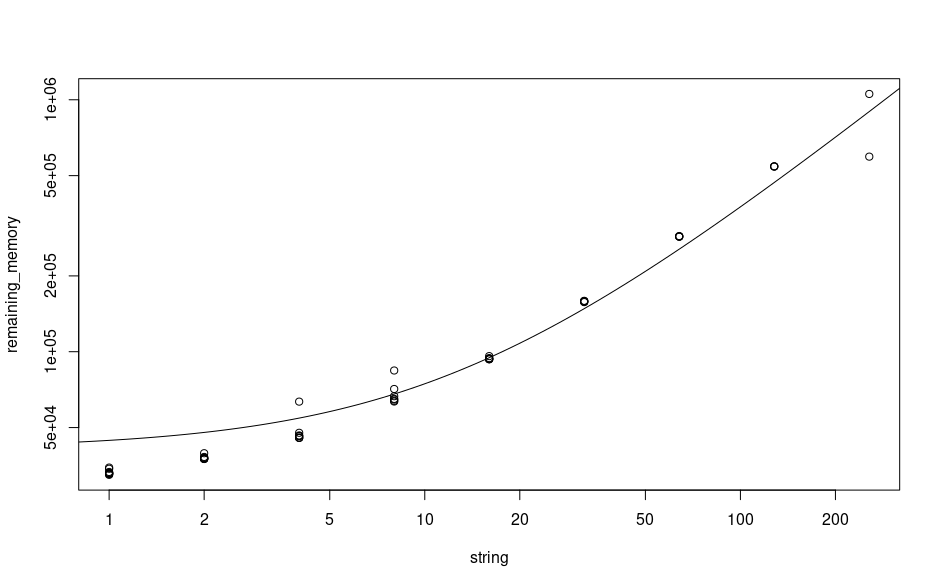
\includegraphics[width=\textwidth]{../proof_of_concept/prediction2.png}
  \caption{A log-log plot comparing the number of characters in a string and the
  observed memory unaccounted by the array. In each column, separate points
  correspond to different array sizes. The curve is a best-fit linear regression
  line.}
  \label{fig:regression1}
\end{figure}

Figure~\ref{fig:regression2} presents a more detailed view, but suggests
the same conclusion. While the predictions seem to consistently overestimate
memory consumption for short strings and similarly underestimate it for longer
strings, adding a quadratic term is not enough to remove the bias in errors, and
the errors are sufficiently small (see Section~\ref{sec:after_adjustments} for
more details).

\begin{figure}
  \centering
  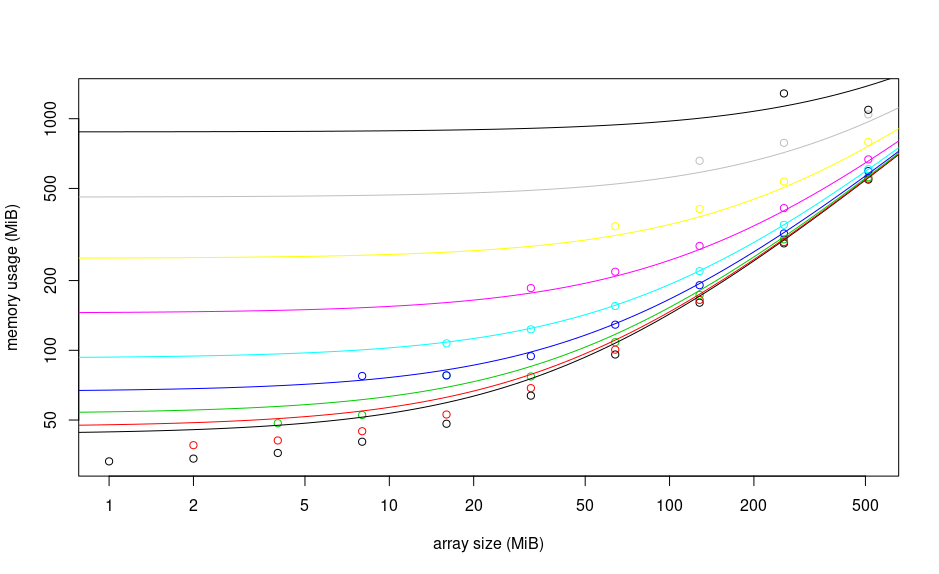
\includegraphics[width=\textwidth]{../proof_of_concept/prediction1.png}
  \caption{A log-log plot showing memory consumption across a range of array
    sizes, with different string sizes represented by different colours. For
    each string size, we also draw a regression line in the corresponding
    colour.}
  \label{fig:regression2}
\end{figure}

\subsection{Adjusted Performance} \label{sec:after_adjustments}

We can use the two numerical parameters in Equation~\eqref{eq:regression} to
adjust our map class in order to ensure that it uses the correct amount
of memory. We run a similar set of experiments as before, except replacing array
size with expected memory usage as one of our independent variables (the other
being string size). Memory usage is set to four different values: 64, 128,
256, and \SI{512}{\mebi\byte} (note that the smallest possible memory usage is
about \SI{40}{\mebi\byte}), while string size is exponentially increased from
\SI{1}{\mebi\byte} up to the largest power of two small enough so that the
string can be constructed from the array. We plot the errors in
Figure~\ref{fig:adjustment}. Note that the largest error is smaller than
\SI{50}{\kibi\byte}, which is good enough for our needs.

\begin{figure}
  \centering
  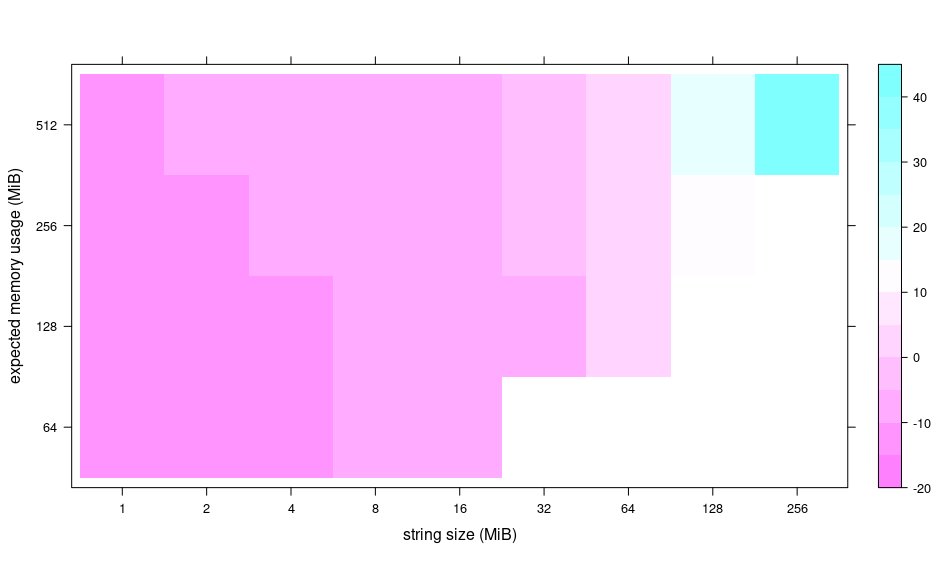
\includegraphics[width=\textwidth]{../proof_of_concept/adjusted.png}
  \caption{A heat map of errors (in \si{\kibi\byte})}
  \label{fig:adjustment}
\end{figure}

\section{Experimental Evaluation}

Experiments were performed in order to determine how well performance metrics
observed with a standalone Java application transfer to MiniShift. We explore
four values of \texttt{memoryUsage} (\SI{64}{\mebi\byte}, \SI{128}{\mebi\byte},
\SI{256}{\mebi\byte}, \SI{512}{\mebi\byte}), while keeping \texttt{cpuTime} at
zero so that each run lasts only as long as it takes to allocate and randomise
the memory. For \texttt{outputSize}, we explore every power-of-two number of
\si{\mebi\byte} compatible with the current \texttt{memoryUsage} value. We stick
to a single component and record CPU and memory consumption at \SI{1}{\second}
intervals using Prometheus. Each \texttt{memoryUsage} and \texttt{outputSize}
configuration is written into \texttt{components.yaml} and run three times. With
each run, we recreate all OpenShift components (pods, services, etc.), wait for
the control server to terminate, and retrieve the generated JSON files.

Figure~\ref{fig:cpu_experiment} shows CPU usage across all runs. Even
though our standalone Java application easily reaches 100\% CPU usage, when
transferred to an OpenShift environment, a typical run could only get around
10\%--15\% (as indicated by the red curve), occasionally reaching up to 70\% or
80\% CPU usage. This can be explained by the fact that MiniShift internal
processes as well as Flink JobManager and TaskManager are all running on the
same machine. Even though the processes are distributed among eight cores, this
overhead is sufficient to significantly decelerate the application.

\begin{figure}
  \centering
  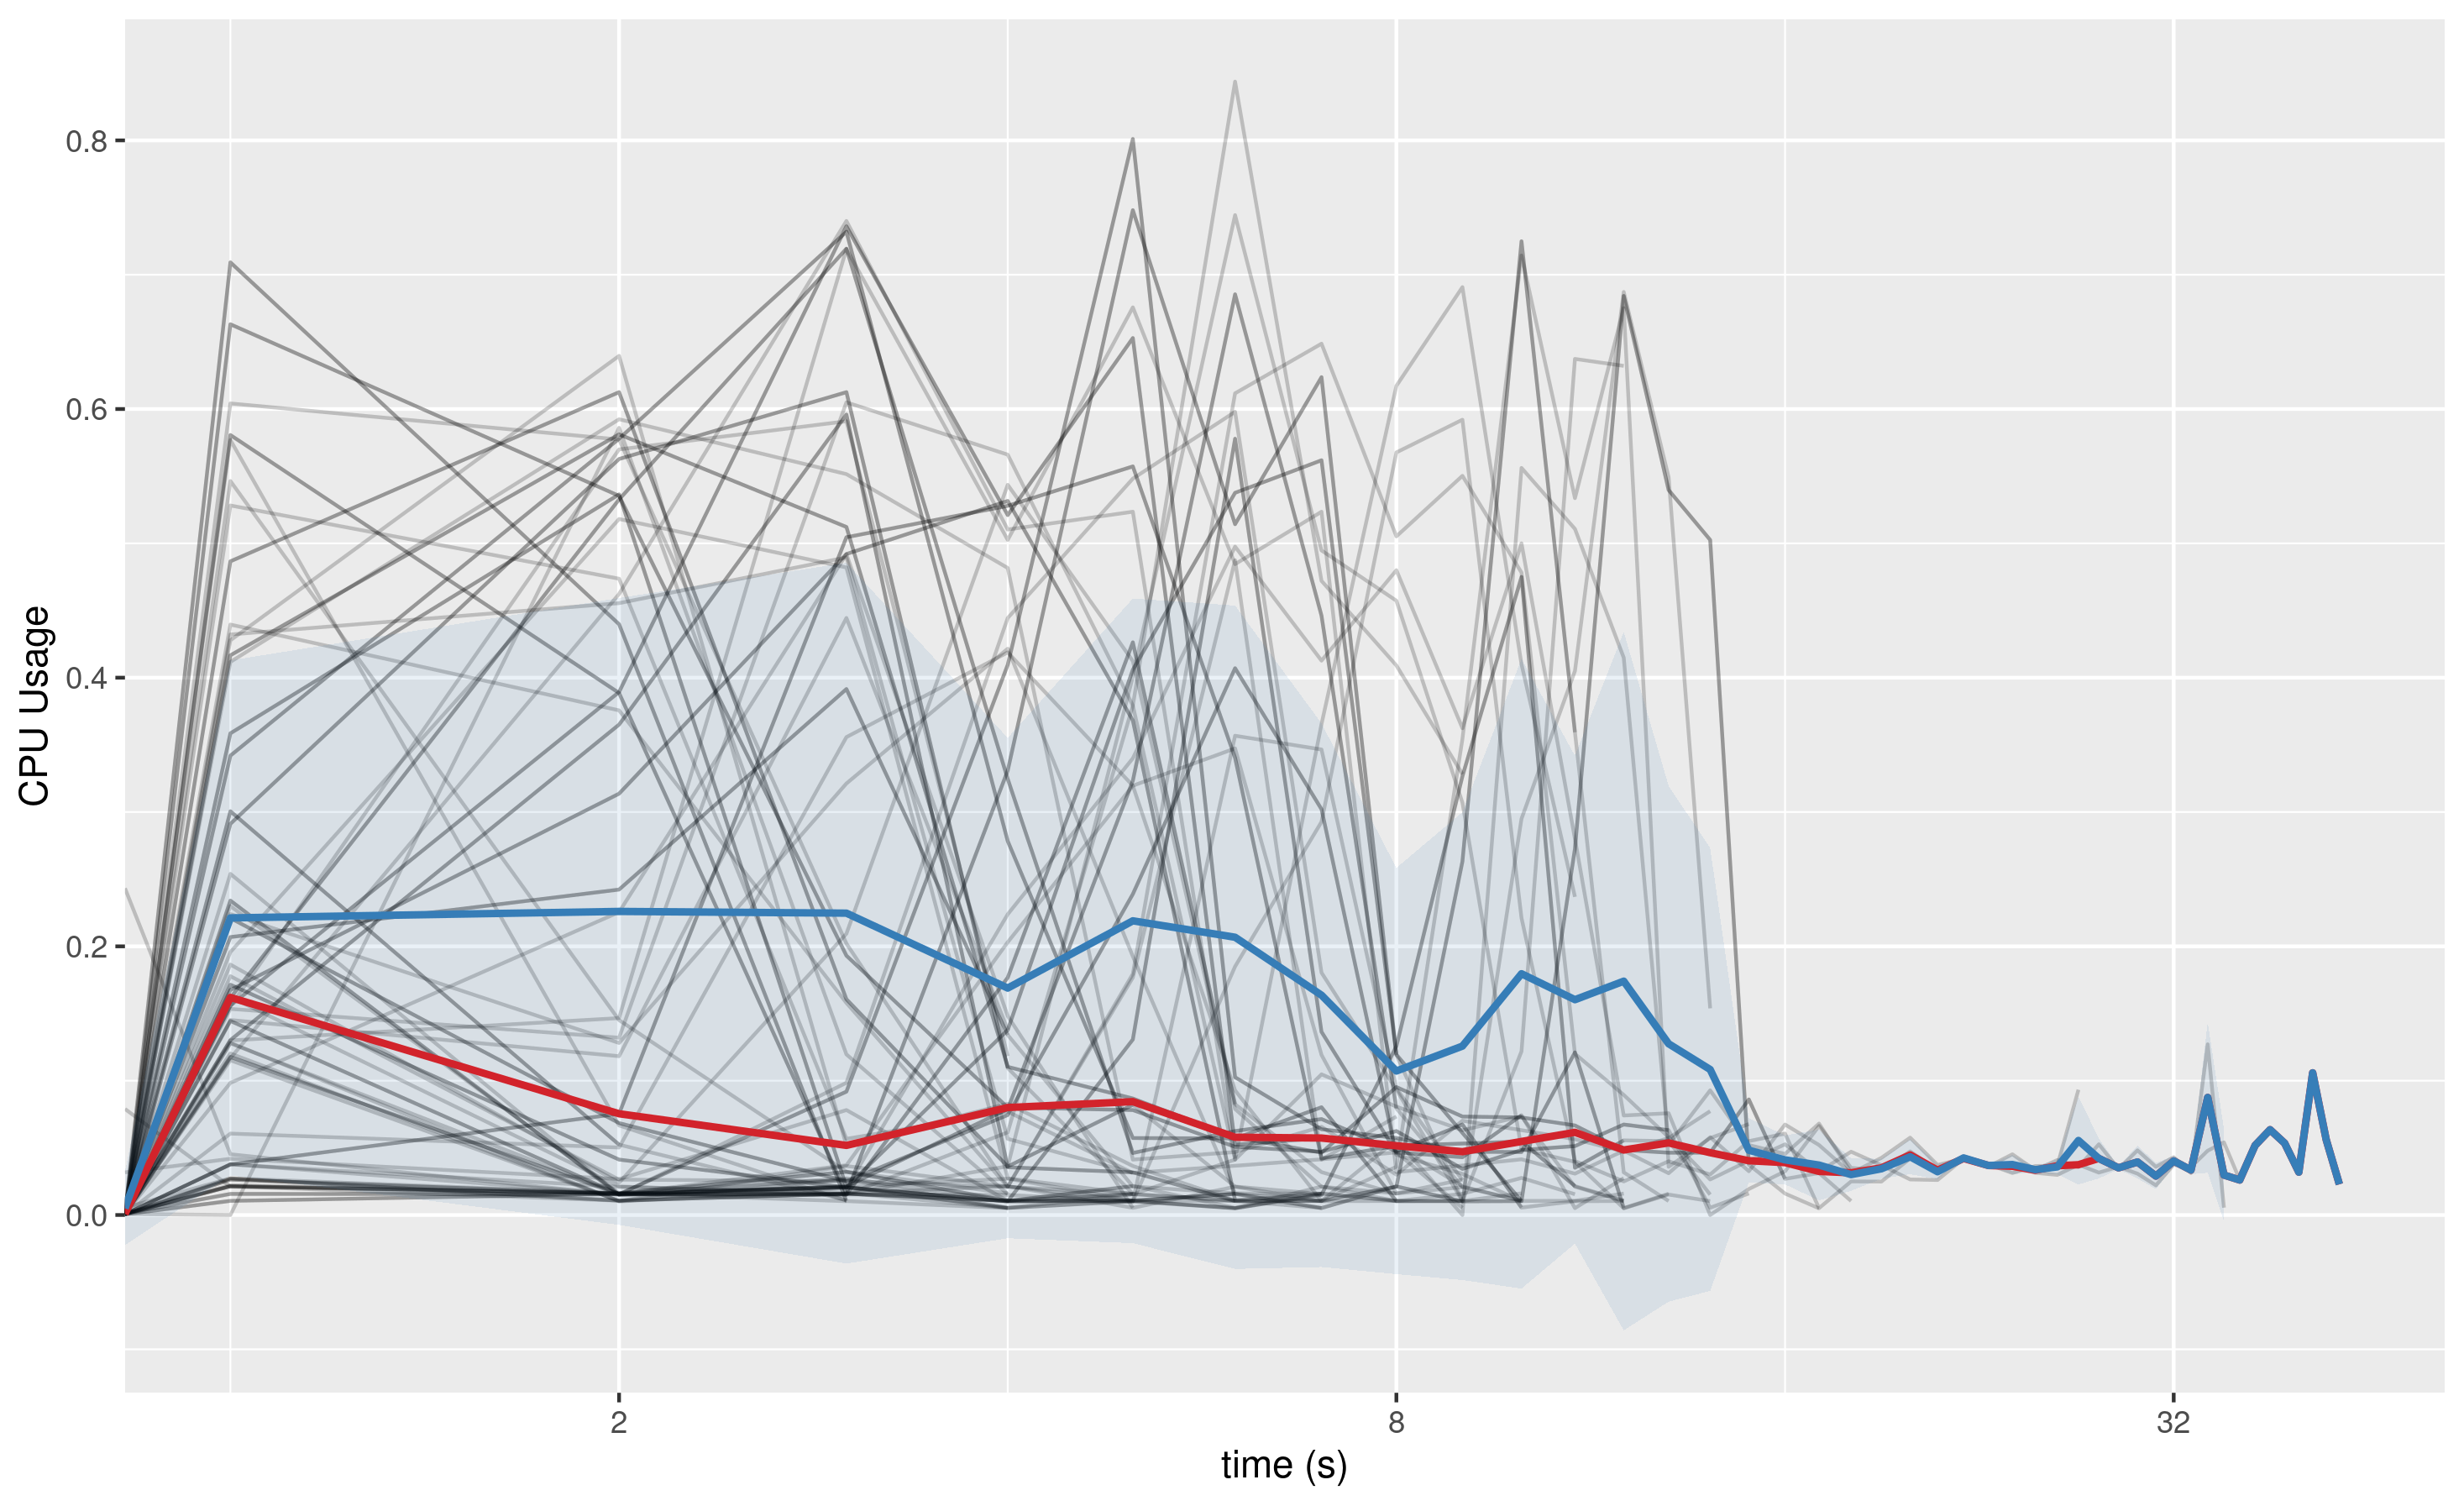
\includegraphics[width=\textwidth]{../plots/cpu_experiment.png}
  \caption{CPU usage across time. Each gray line represents a different run. The
  red curve is their (pointwise) median, the blue curve is the mean, while the
  shaded area marks one standard deviation around the mean. Note that time is on a
  $\log$ scale.}
  \label{fig:cpu_experiment}
\end{figure}

Figure~\ref{fig:heap_experiment} shows similar memory usage measurements divided
into four plots, one for each value of \texttt{memoryUsage}. We can see that
there is significant variation among runs (and different \texttt{outputSize}
values). In fact, in order to determine whether memory usage is optimal or
hampered, one would need to run many identical experiments to account for
variability. Moreover, each curve is unlikely to be fully summarised by a single
number: maximum values are almost always higher than the expected result, while
means are likely to be distorted by the initial several seconds of low memory
usage as well as observed dips in memory usage later in the execution.

Note that individual runs can be summarised as follows:
\begin{enumerate}
\item Memory usage starts low.
\item It rises two times.
\item Sometimes memory usage experiences a significant drop, and sometimes this
  step is skipped.
\item Memory usage stays constant for a while.
\item The process terminates.
\end{enumerate}

We can easily explain this pattern. The first increase is caused by the array
allocation, while the second one is the result of constructing the output
string. The drop in memory usage happens when the array is deallocated
(garbage-collected) some time after the execution of my code completes.
Sometimes that happens early enough to be captured by Prometheus, and sometimes
the Flink job is marked as complete before garbage collection activates.

\begin{figure}
  \centering
  \begin{subfigure}[t]{0.49\textwidth}
    \centering
    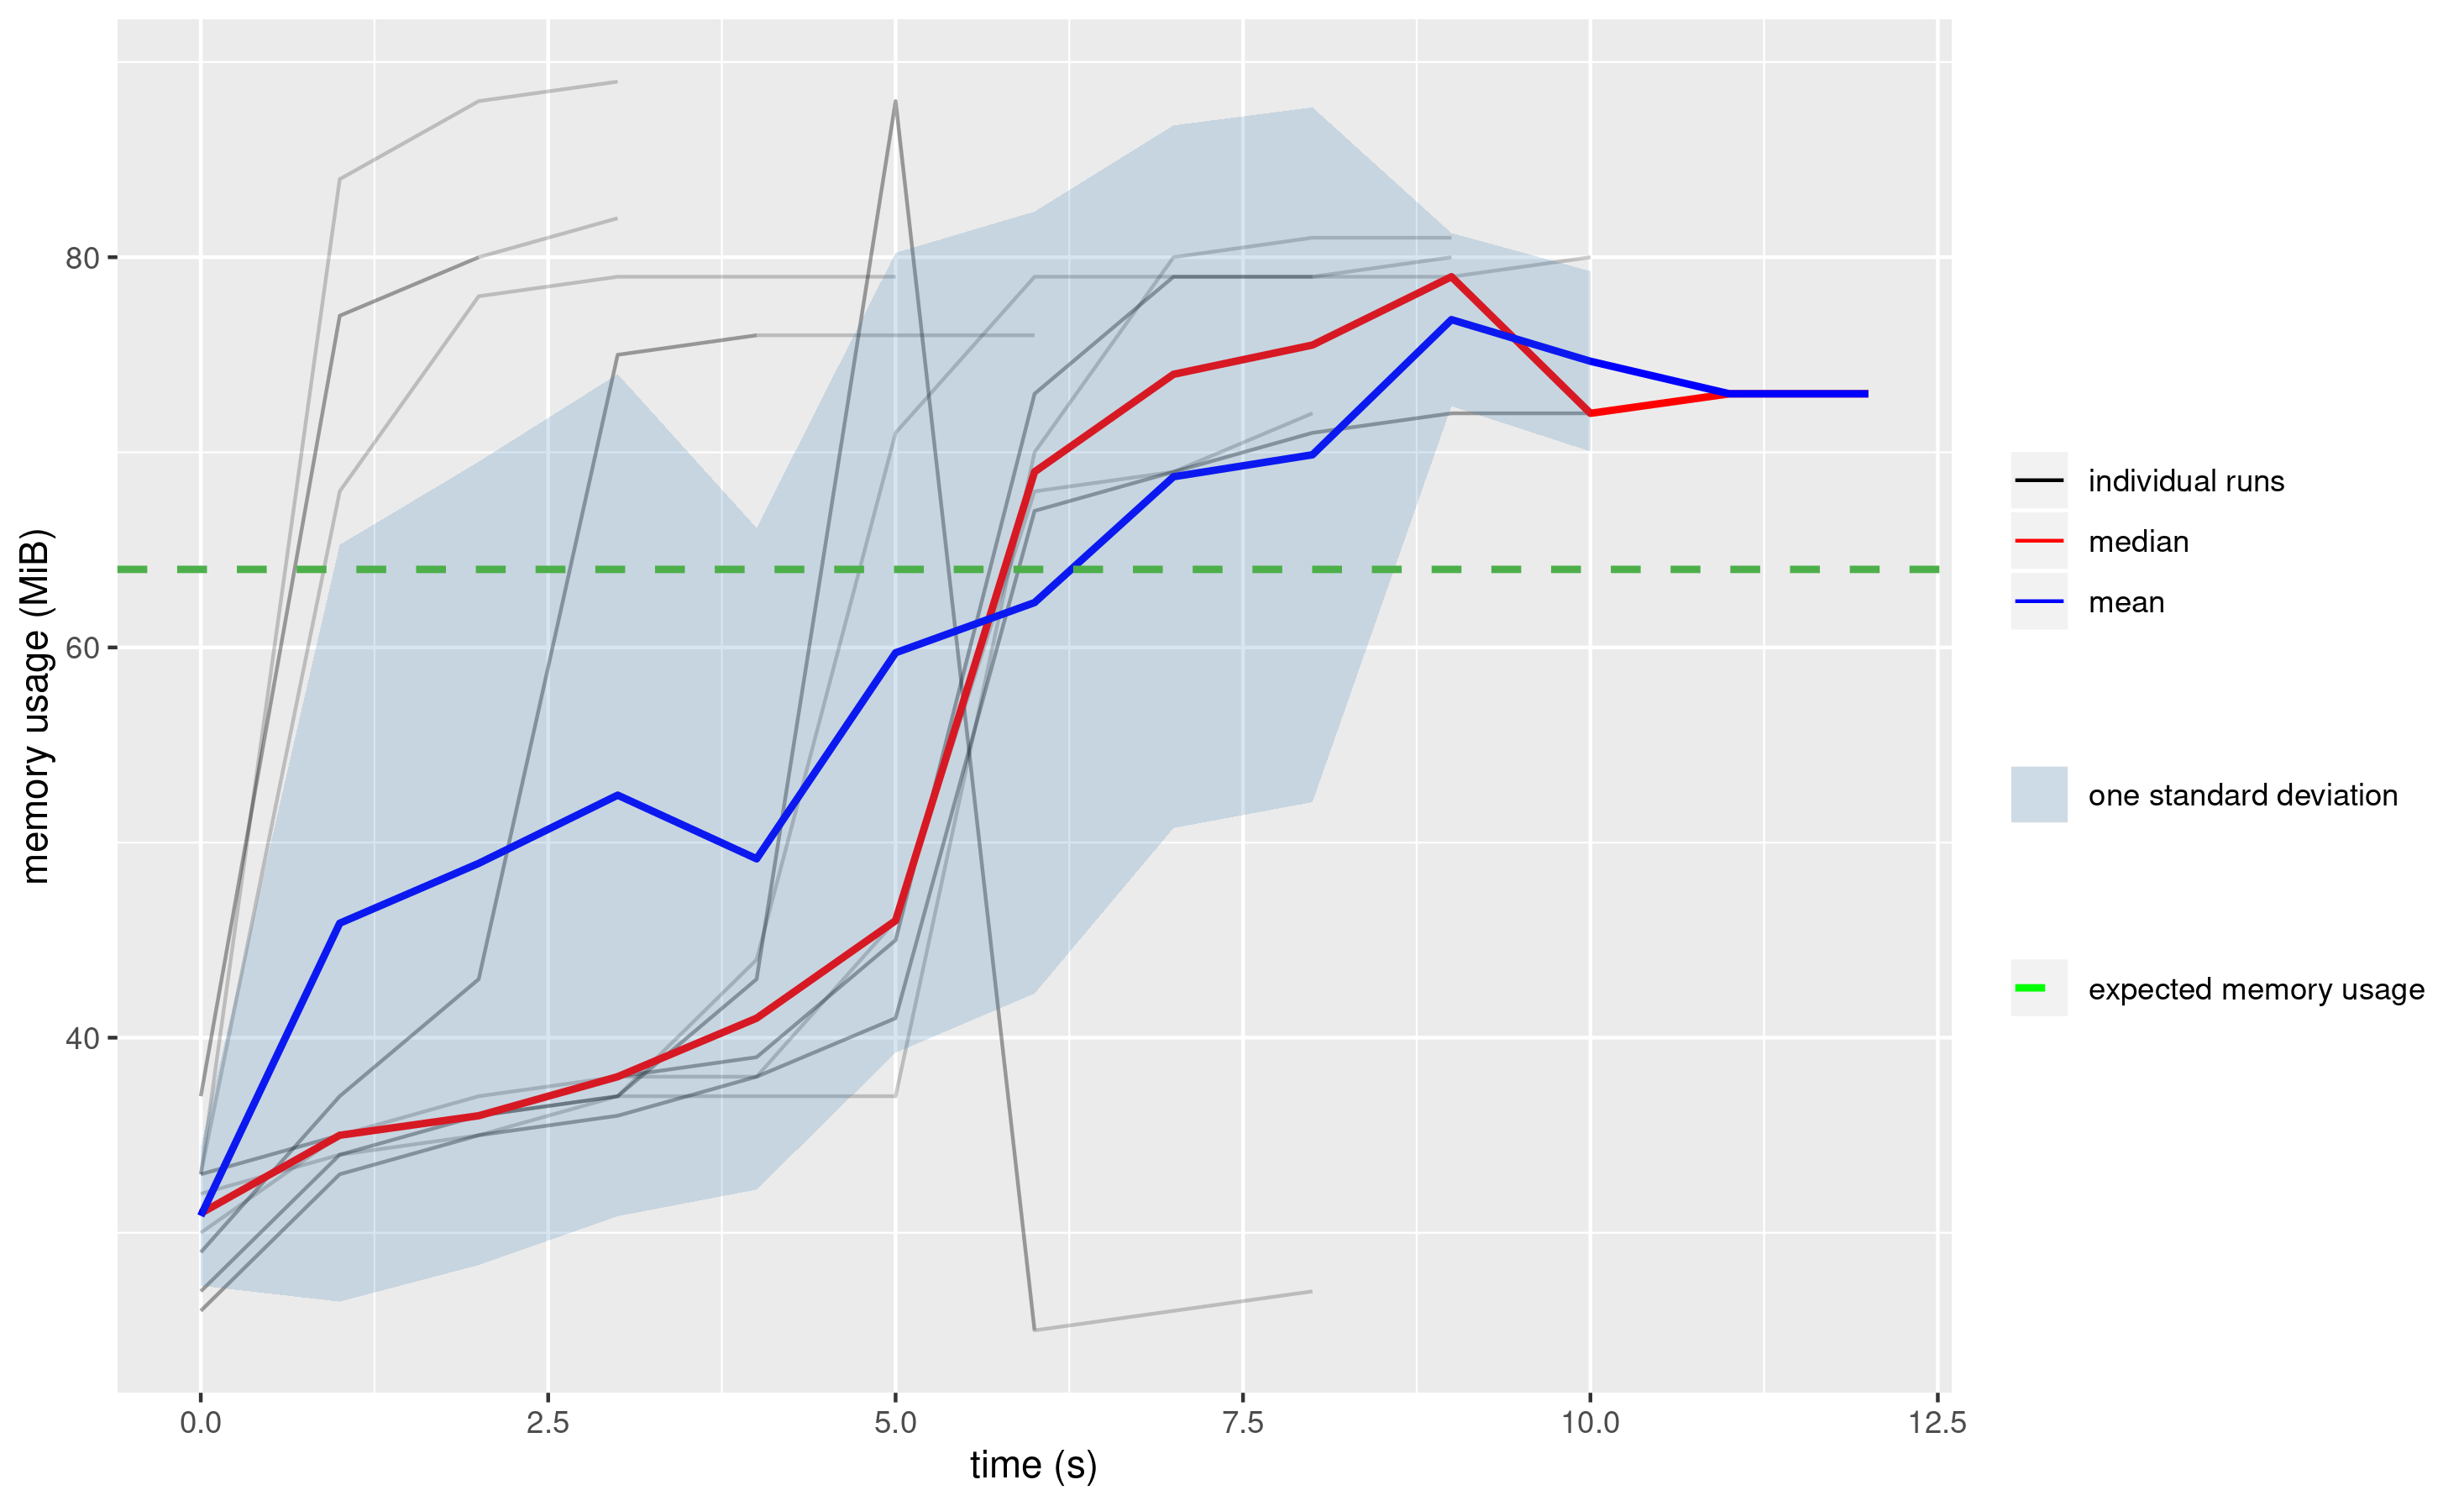
\includegraphics[width=\textwidth]{../plots/heap_64.png}
    \caption{expected heap usage: \SI{64}{\mebi\byte}}
    \label{fig:heap_64}
  \end{subfigure}
  \begin{subfigure}[t]{0.49\textwidth}
    \centering
    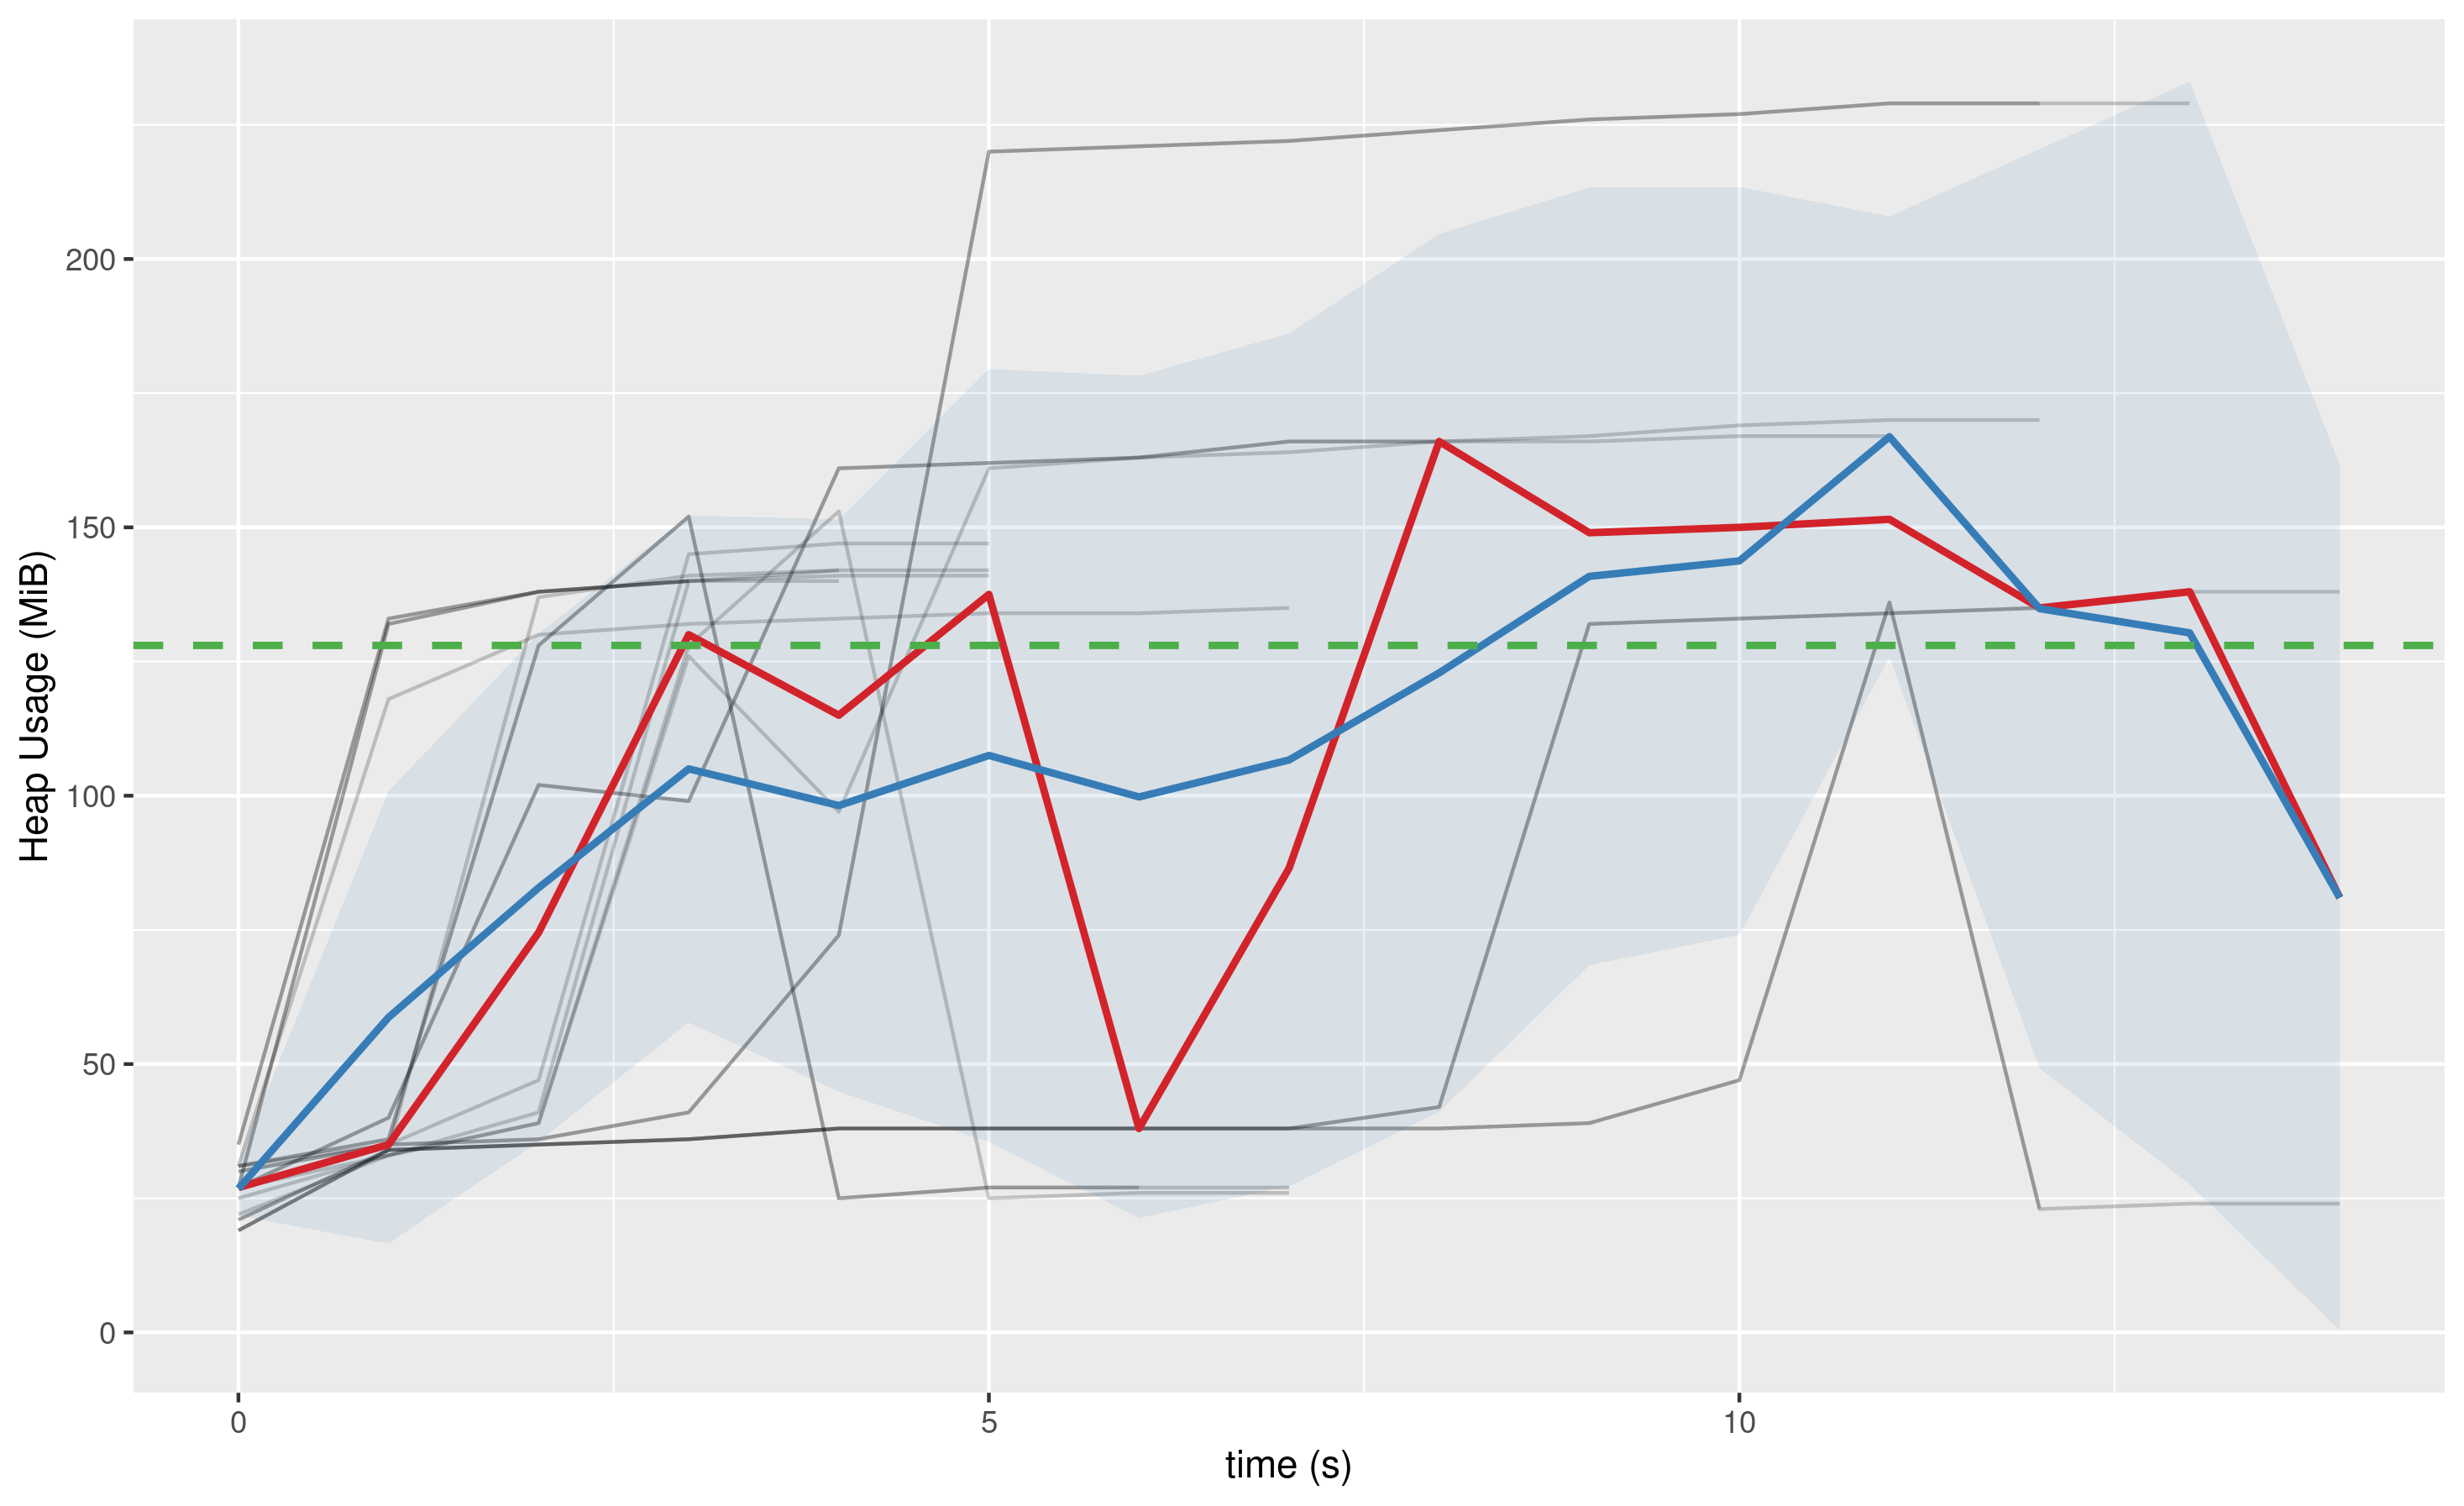
\includegraphics[width=\textwidth]{../plots/heap_128.png}
    \caption{expected heap usage: \SI{128}{\mebi\byte}}
    \label{fig:heap_128}
  \end{subfigure}
  \begin{subfigure}[t]{0.49\textwidth}
    \centering
    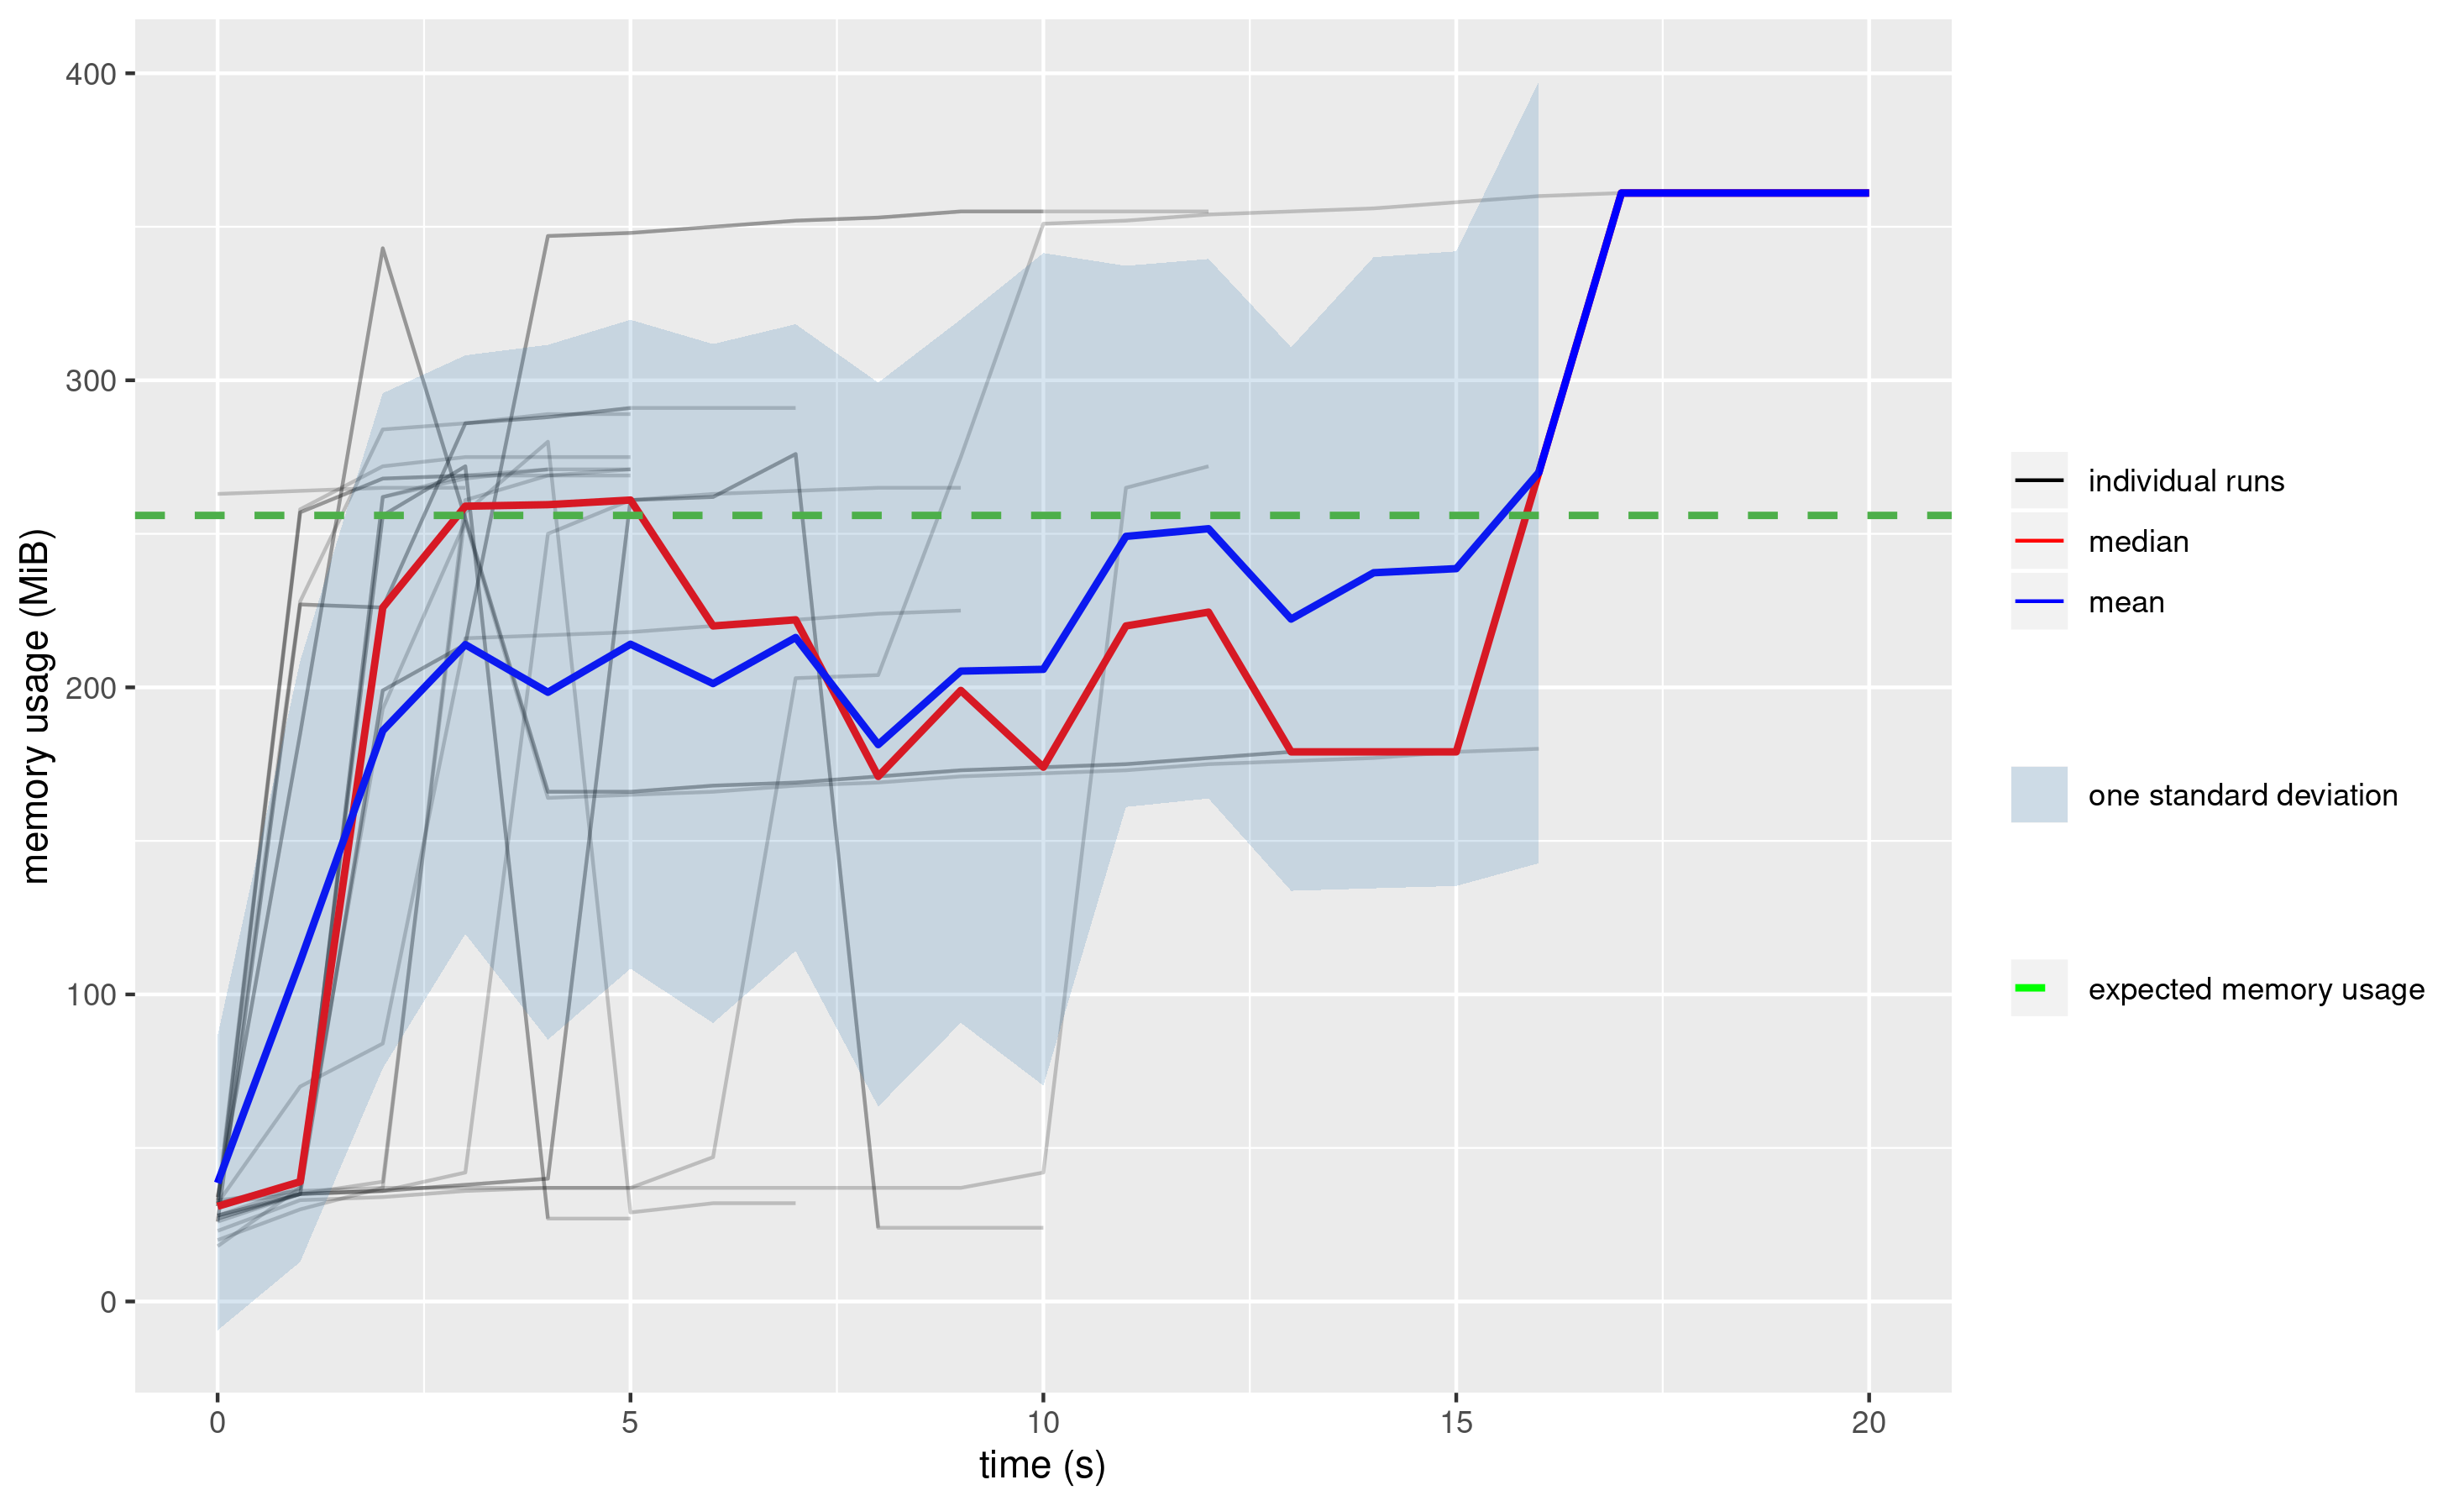
\includegraphics[width=\textwidth]{../plots/heap_256.png}
    \caption{expected heap usage: \SI{256}{\mebi\byte}}
    \label{fig:heap_256}
  \end{subfigure}
  \begin{subfigure}[t]{0.49\textwidth}
    \centering
    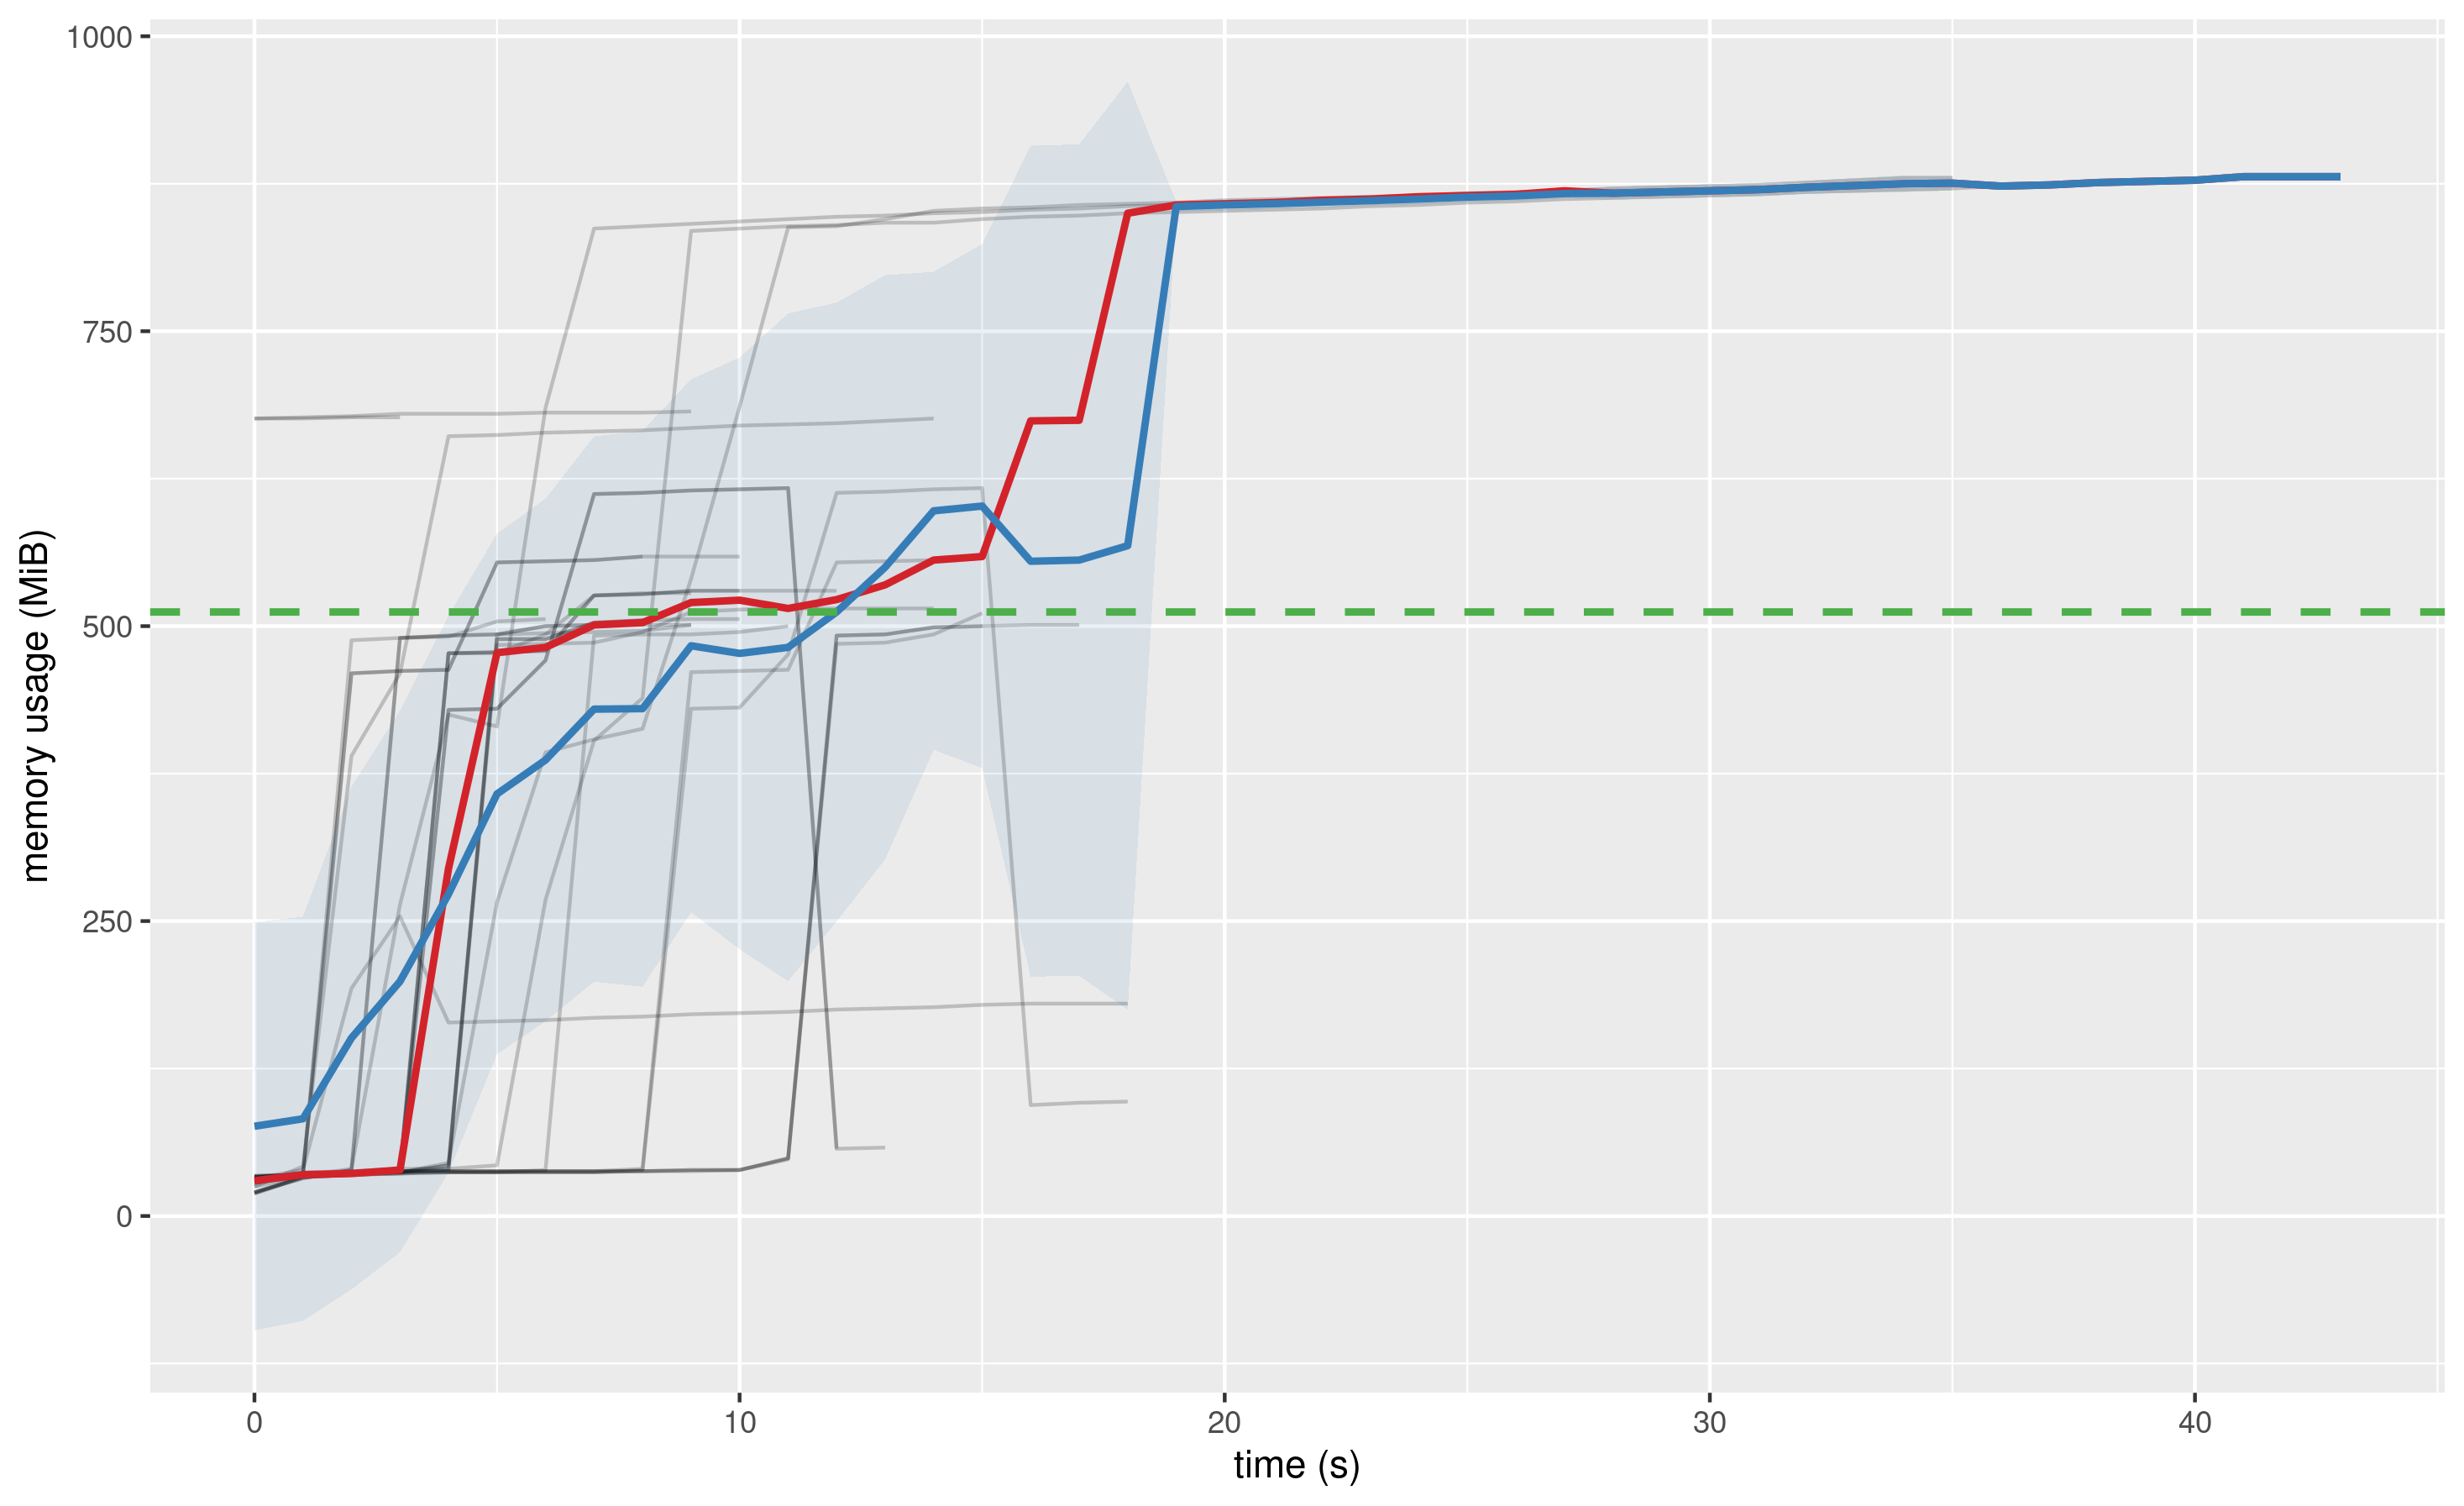
\includegraphics[width=\textwidth]{../plots/heap_512.png}
    \caption{expected heap usage: \SI{512}{\mebi\byte}}
    \label{fig:heap_512}
  \end{subfigure}
  \caption{Observed versus expected memory usage across time for four expected
    memory amounts. The green dashed horizontal line marks the expected amount
    of memory usage. Each gray line represents a different run. The red curve is
    their (pointwise) median, the blue curve is the mean, while the shaded area
    marks one standard deviation around the mean.}
  \label{fig:heap_experiment}
\end{figure}

Finally, we consider the extent to which memory usage can be summarised by
taking the maximum across time. We report each difference between expected $E$
and observed $O$ values as a relative error, i.e.,
\[
  \frac{O - E}{E}.
\]
We consider these errors for all viable combinations of \texttt{memoryUsage} and
\texttt{outputSize} and report the median of the three identical runs performed
on each combination. The results are in Figure~\ref{fig:relative_errors}.
Unsurprisingly, maximum memory usage across time is usually higher than the
estimate. Also note that the overall shape of the heat map is similar to
Figure~\ref{fig:adjustment}, where we measure differences between observed and
expected memory usage with the standalone Java application. In both cases,
observed values are smaller with lower values of \texttt{outputSize}, and a
combination of high overall memory usage and a long output string in the top
right corner of both heat maps is likely to result in observed memory usage
being significantly higher than the expected value. Even though we take median
values to reduce the effect of outliers, observed memory usage can be up to 80\%
higher than the expected value, adding evidence to the imprecision and
unreliability of making judgments based on a single number or a single
experiment.

\begin{figure}
  \centering
  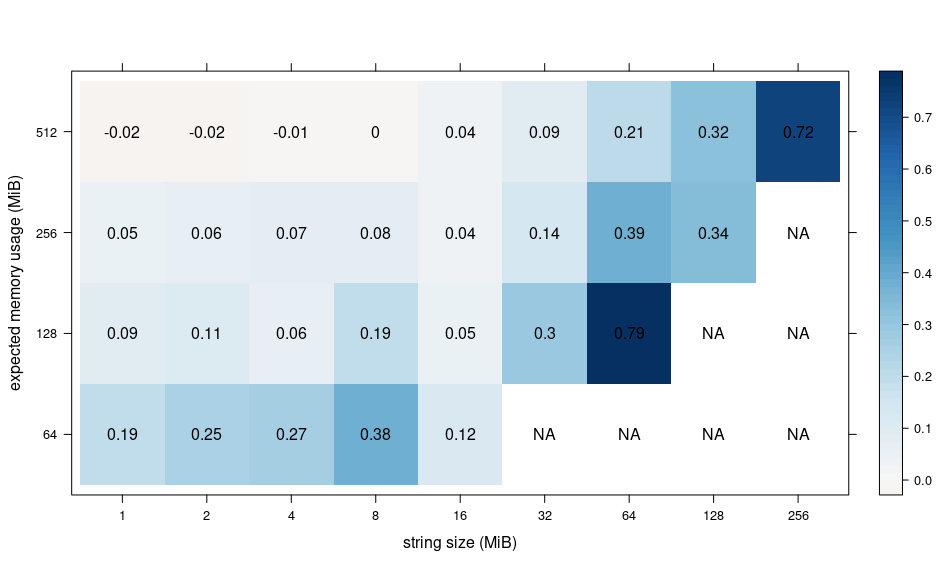
\includegraphics[width=\textwidth]{../plots/relative_median_errors.png}
  \caption{Relative median memory usage errors, as predicted by the maximum
    memory usage across execution}
  \label{fig:relative_errors}
\end{figure}

\section{Example Applications}

\subsection{A Simple Website}

\begin{table}
  \centering
  \caption{Performance statistics of the top 100 e-commerce websites}
  \begin{tabular}{l c c c}
    \toprule
    Metric & min & mean & max \\
    \midrule
    Page load time (\si{\second}) & \tablenum{0.468} & \tablenum{2.67} & \tablenum{9.67} \\
    Page size (\si{\mebi\byte}) & \tablenum{0.719} & \tablenum{3.03} & \tablenum{14.21} \\
    Number of requests made per load & \num{45} & \num{192} & \num{660} \\
    \bottomrule
  \end{tabular}
  \label{tbl:web}
\end{table}

In order to simulate a website, we need some data about the performance metrics
of a typical website. We extract the data in Table~\ref{tbl:web} from
experiments run on popular websites \cite{web_performance}. Thus, we can
simulate an average website with a single component by making the following
modelling assumptions:
\begin{itemize}
\item $\texttt{cpuTime} = \frac{\text{page load time}}{\text{number of requests
      per load}} = \frac{\SI{2.67}{\second}}{192} \approx \SI{0.014}{\second}$;
\item \texttt{memoryUsage} is minimal, i.e., the smallest amount necessary to
  construct the output string;
\item $\texttt{outputSize} = \frac{\text{page size}}{\text{number of requests
      per load}} = \frac{\SI{3.03}{\mebi\byte}}{192} = \SI{16.16}{\kibi\byte}$;
\item $\texttt{requestsPerMessage} = \text{number of requests per load} = 192$.
\end{itemize}

\subsection{A Machine Learning System}

\section{Input/Output Simulation}

% TODO: how do we know NODE_SIZE

In order to simulate input/output (I/O) interactions similar to accessing a
database or reading a file, we introduce a number of new component-specific
parameters:
\begin{description}
\item[$\texttt{databaseOnStartup} = \text{true}$] means that I/O will be
  simulated only once, during the initialisation stage. Otherwise it will be
  simulated with every call to \texttt{map()}.
\item[\texttt{numRequests}] is the number of request-response interactions
  between the component and the (simulated) data source.
\item[\texttt{responseSize}] is the size of the response (in \si{\mebi\byte}).
\item[\texttt{databaseLatency}] is the amount of time spent between a request
  and receiving the first byte of the response (in \si{\milli\second}).
\item[\texttt{bandwidth}] is the bandwidth for transferring the response (as the
  request is assumed to be small) (in \si[per-mode=symbol]{\byte\per\second}).
\item[\texttt{intervalBetweenRequests}] is the amount of time between receiving
  a response and sending another request (in \si{\milli\second}).
\end{description}
We can then use these variables to simulate an I/O dialogue as described in
Algorithm~\ref{alg:io} (with unit conversion and rounding operations skipped for
simplicity). We use a linked list $L$ to gradually construct an object of size
\texttt{responseSize}, simulating a big file slowly being uploaded to memory.
Setting the size of a single linked list node as \texttt{NODE\_SIZE} allows us
to calculate that we need $\frac{\texttt{responseSize}}{\texttt{NODE\_SIZE}}$
nodes in order to simulate a file transfer of size \texttt{responseSize}.
Similarly, in order to achieve the right \texttt{bandwidth}, we need each node
to be constructed in $\frac{\texttt{NODE\_SIZE}}{\texttt{bandwidth}}$ time (we
are assuming that adding a random integer to a list takes a negligible amount of
time).

\begin{algorithm}
  \SetKwData{numRequests}{numRequests}
  \SetKwData{databaseLatency}{databaseLatency}
  \SetKwData{responseSize}{responseSize}
  \SetKwData{nodeSize}{NODE\_SIZE}
  \SetKwData{bandwidth}{bandwidth}
  \SetKwData{intervalBetweenRequests}{intervalBetweenRequests}
  \SetKwFunction{sleep}{sleep}
  \SetKwFunction{LinkedList}{LinkedList}
  \SetKw{new}{new}
  \For{$i \leftarrow 1$ \KwTo \numRequests}{
    \sleep{\databaseLatency}\;
    $L \leftarrow$ \new \LinkedList of integers\;
    \For{$j \leftarrow 1$ \KwTo $\frac{\responseSize}{\nodeSize}$}{
      add a random integer to $L$\;
      \sleep{$\frac{\nodeSize}{\bandwidth}$}\;
    }
    \If{$i < \numRequests$}{
      \sleep{\intervalBetweenRequests}\;
    }
  }
  \caption{Simulation of a slow network data transfer}
  \label{alg:io}
\end{algorithm}

\bibliographystyle{abbrv}
\bibliography{report}
\end{document}